%!TEX root = main.tex

\section{System overview}
\label{sec:system}

\subsection{Crowdsourced live video system architecture}
\label{sub:system-architecture}
The architecture of the crowdsourced live video system is shown in Figure~\ref{fig:system}. The system consists of five parts: controller, camera, front-end relay server, viewer, and storage system. Consumers mainly make two actions on this system: post and watch video. 
%We use Cassandra cluster as our storage system. Cassandra is an key-value based open source distributed storage system which has been deployed in many large Internet company, such as Google, Facebook and Amazon~\cite{Beernaert2013cassandra}. It provide high availability and support clusters spanning multiple datacenters. 
\begin{figure}[ht]
	\centering
	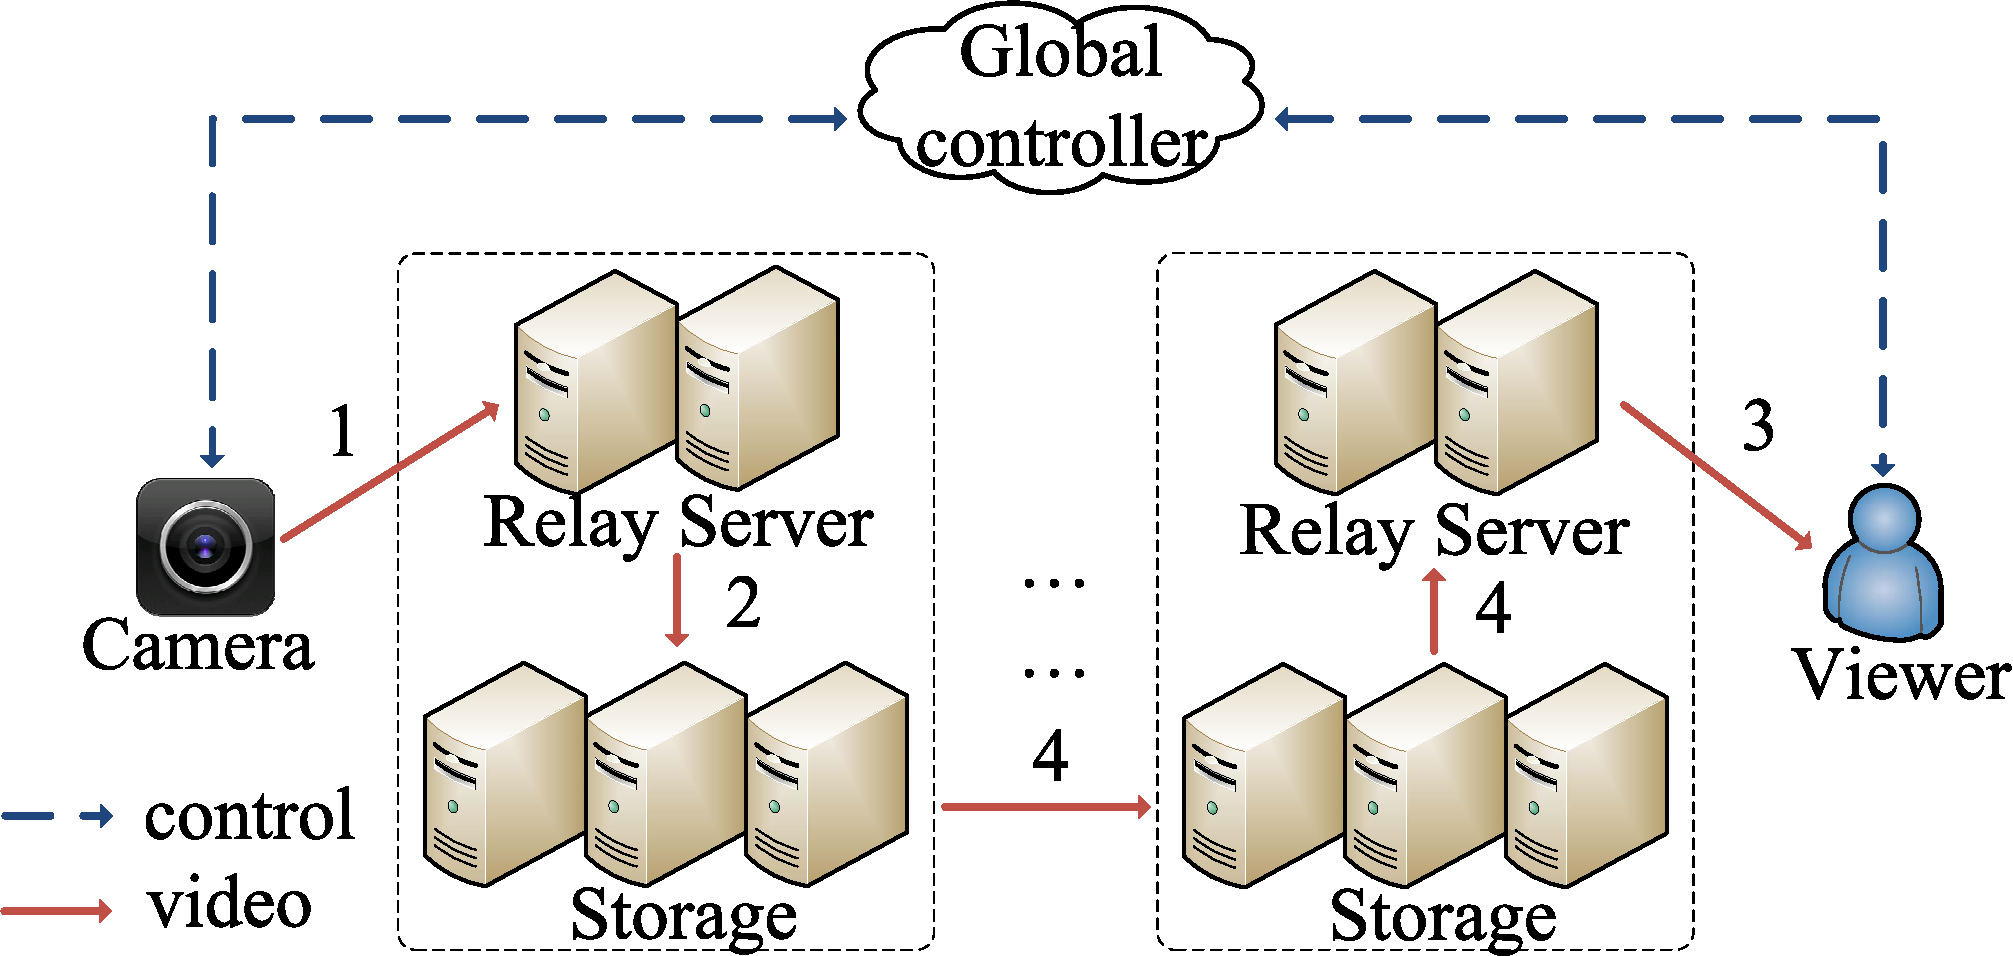
\includegraphics[width=3.5in]{system-new}
	\caption{An overview of the crowdsourced live video system.}
	\label{fig:system} 
	\termspace
\end{figure}

\textbf{\textit{Post video:}} When consumers want to post a video, camera will first connect to the controller. The controller will select a best front-end server for it according the camera's location and network condition. Ganjam \etal~\cite{ganjam2015c3} find that a centralized control plane can improve the video quality in video broadcast platform. Cameras set up TCP connection 1 with the 'pick up' front-end server. The front-end server play two kinds of role: publisher and subscriber. Publishers receive the video from camera and the subscriber send video to viewers. After receiving the video from camera the publisher will set up TCP connection 2 to send the video to storage servers which is in the same DCN(Data Center Network) with the front-end servers. 

\textbf{\textit{Watch video:}} When viewers want to watch a video, they also first connect to the controller. The controller will select the neareast front-end server which is also in the same ISP(Internet Service Provider) with consumer. Viewers set up TCP connection 3 with the 'pick up' front-end to request a live video. And then the front-end server will set up  TCP connection 4 to fetch the video from storage server. If the front-end server and video are in the same DCN, it will fetch the video directly. However, if the video is stored in other DCN, the front-end sever will fetch the video from remote DCN. Those DCNs in our system is connected directly by optical fiber which has a large bandwidth and short RTT. The front-end sever will cache the video temporarily that it is playing. When other consumers request the same video, the front-end servers will send back the video that is cached in it which make it unnecessary to fetch from storage servers. Such caching video solution makes our system scalable as even thousands of consumers request a same video, the front-end sever just needs to fetch the video only once.

In totally, the crowdsourced live video system set up four TCP connections for a single live video watching process. The connections 2 and 4 are between front-end server and storage server and they both go through internal network which has low packet loss rate and short RTT. Connections 1 and 3 : camera between front-end sever and front-end sever between viewers go through WAN(wide area network) which has high packet loss rate and long RTT. In Section~\ref{sec:system-measurement} we will analysis the whole system based on the TCP connections, especially the influence caused by the two connections in unstable WAN.

%This is different from traditional live video system. When the traditional live video system broadcast a football game, the camera will transport the video to the front-end server and the front-end server will immediately deliver it to the CDN(Content Dilivery Network) both by stable internal network. As the video is delivered by stable internal netowrk, the traditional live video system has more stable video supply compared with crowdsourced live video system. And that also means that in traditional live video system the network factors that influence user experience is mainly on the connection between Apps and front-end server. However, in crowdsourced live video system the unstable connection between camera and front-end sever may also influence the system. 
  
\subsection{Overview of video frame}
\label{sub:video-frame}
The video codec in our system is H.264 and we use RTMP(Real Time Messageing Protocol, which is based on TCP) ~\cite{zambelli2009iis}to transfer video. In H.264 there are four kinds of frame to produce a video: I frame, P frame, B frame and V frame. I frame is IDR(Instantaneous Decoder Refresh) frame, which is known as a keyframe and can build a without any other information ~\cite{timothy2011h264}.  P frame is Predicted frame which predicts the picture according the previous frame. B frame is Bidirectional predicted frame which predicts picture according the previous or future frame. In this paper, we do not distinguish P frame and B frame and call them both as P frame. V frame is the voice frame which records the voice along the video. The size and produced terminal of frame are different. I frame is often 10-100K bytes and is produced every 4 seconds. P frame is often 2-10K bytes and its produced terminal is unstable, changed according the dynamic of the video. The size of V frame is less than 1K bytes and our system produces 25 V frames every second. Different frames may have different performance in network. In Section~\ref{sec:frame-analysis} we will detail the different performance of each type of frame.


%For timeless storage and fetching the video, the storage unit in our Cassandra cluster is frame. Which means the system uses a key to storage and fetch echa frame.  

\iffalse
\begin{figure}[ht]
	\centering
	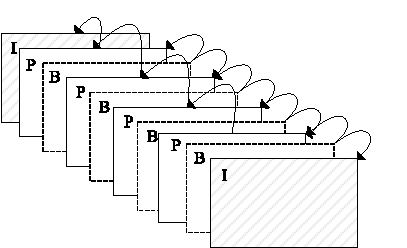
\includegraphics[width=2.5in]{frame}
	\caption{An overview of H.264 frame.}
	\label{fig:frame}
	\termspace
\end{figure}
\fi


 

